In this chapter a search for highly ionizing, short tracks is presented. The chapter will be structured as follows:
In \mbox{Sec.~\ref{sec:Motivation}} a motivation will be given, followed by an overview of the general search strategy in \mbox{Sec.~\ref{sec:GeneralSearchStrategy}}.
As the variable \dedx plays a crucial role in this analysis, a general introduction and different possible parametrizations will be introduced in \mbox{Sec.~\ref{sec:DeDxMeasurement}}.
In this context also the conducted offline calibration of the silicon pixel detector will be explained.
After presenting the simulated SM and signal samples which were used in this analysis (\mbox{Sec.~\ref{sec:SimulatedSamples}}) the event selection is shown (Sec.~\ref{sec:EventSelection}).
Then, the various sources of background are charecterized (Sec.~\ref{sec:SourcesOfBackgrounds}) and the methods to estimate their size are presented (\ref{sec:BackgroundEstimation}).
As a final step an optimization in the search sensitivity was done, which can be found in Sec.~\ref{sec:Optimization}.
The chapter concludes by presenting the results of this analysis in Sec.~\ref{sec:Results}, and after a short introduction to the statistical methods of limit setting (Sec.~\ref{sec:LimitSetting}), the results will be interpreted in the context of Supersymmetry (Sec.~\ref{sec:Interpretation}).


%%%%%%%%%%%%%%%%%%%%%%%%%%%%%%%%%%%%%%%%%%%%%%%%%%%%%%%%%%%%%%%%%%%%%%%%%%%%%%%%%%%%%%%%%%%%%%%%%%%%%%%%%%%%%%%%%%%%%%%%%%%%%%%%%%%%%%%%%%%%%%%%%%%%%%%%%%%%%%%%%%%%%%%%%%%%%%%%%%%%
\section{Motivation}
\label{sec:Motivation}
As it was already pointed out in Chap.~\ref{ch:Theory}, Supersymmetry is able to offer solutions to unexplained phenomena in astrophysics and can solve the shortcomings of the Standard Model of particle physics.
Unfortunately, due to the unknown mechanism of supersymmetry breaking, the most general parametrization of Supersymmetry introduces over 100 new dimensions which opens up an incredibly huge phenomenalogically rich space, 
leading to very different possible signature at particle colliders. 
During the Phase\,I run at the LHC in 2012, a variety of different seaches, optimized on the hunt for supersymmetry were conducted.
At the CMS and at the ATLAS experiment, taking data from proton-ptoton collsions, a strong focus was put on the search for hints of SUSY in the strong production sector (e.g. \cite{bib:CMS:RA2_8TeV,bib:CMS:MT2_8TeV,bib:ATLAS:JetPlusMET_8TeV}).
This led already to a wide exclusion in SUSY space, which nevertheless still offers some very interesting non-excluded parameter regions.
The search for SUSY in more "exotic" regions gains therefore more and more attention. 
Typical SUSY scenarios which are not easily excluded by the general SUSY searches consists of so-called compressed spectra, where two or more particles are nearly degenerate in their masses.
When mother and daughter particles are almost mass-degenerate, the remaining decay product in a two body decay can be very soft in \pt, making those scenarios very challenging to search for.
Thus supersymmetric scenarios with compressed spectra are usually much weaker constrained than the corresponding scenarios without compressed spectra.\\

In this analysis the focus is put on the possiblity of a lightest chargino ($\chi^{\pm}_1$) which is almost mass degenerate with the lightest neutralino ($\chi^{0}_1$).
As shown in Sec.~\ref{theorySUSY}, long lifetimes are possible for various reasons.
The scenarios presented here lead to long lifetimes of the chargino because of phase space supression.

A chargino can be produced via chargino pair production through a photon or a Z boson exchange. The chargino decays then via a virtual W boson to the lightest neutralino and fermion-fermion pair (e.g. a pion).
This process is illustrated in the Feynman diagram shown in fig. \ref{fig:FeynmanDiagram}.

\begin{figure}[!tb]
  \centering 
  \begin{tabular}{c}
    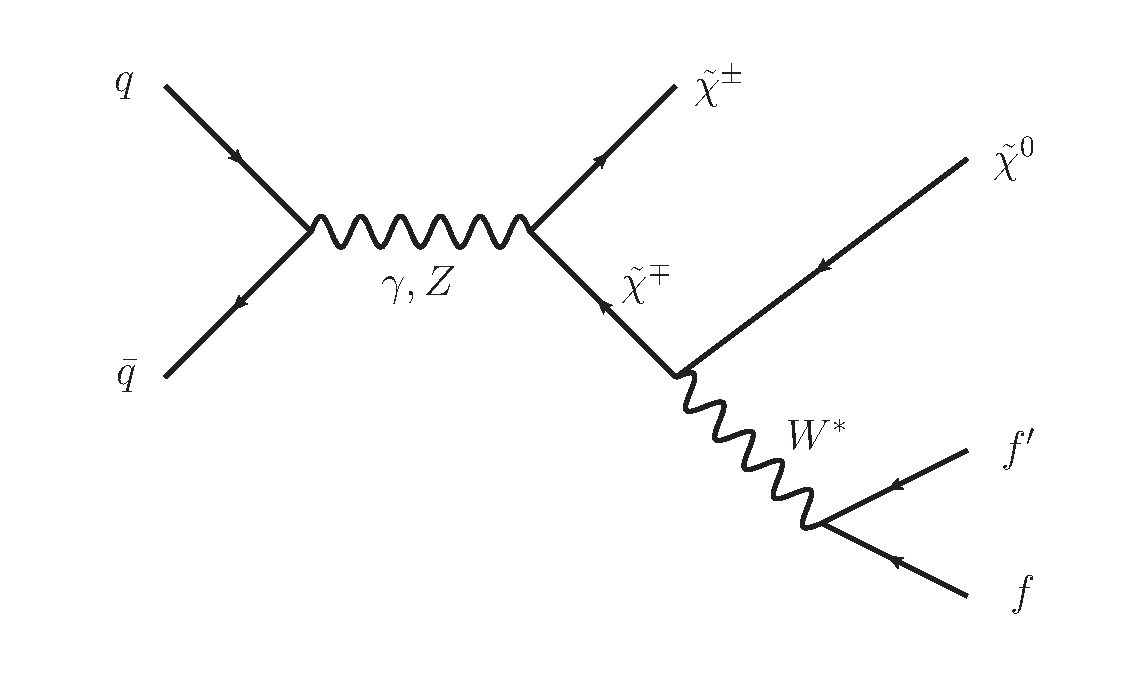
\includegraphics[width=0.75\textwidth]{figures/analysis/ChiChi_ProductionAndDecay.pdf}
  \end{tabular}
  \caption{Feynman diagram showing a possible production mechanism of a chargino pair and the decay channel of a chargino.}
  \label{fig:FeynmanDiagram}
\end{figure}

Other possible production channels are the exchange of a supersymmetric Higgs boson or via a t-channel squark exchange. 
The corresponding Feynman diagrams for the tree level production channels are shown in Fig.~\ref{fig:FeynmanDiagramProductionCharginoPair}.

\begin{figure}[!b]
  \centering 
  \begin{tabular}{c}
    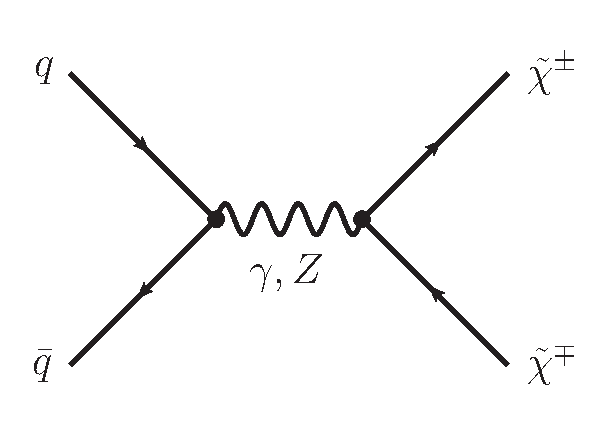
\includegraphics[width=0.33\textwidth]{figures/analysis/ChiChi_GammaZ.pdf}
    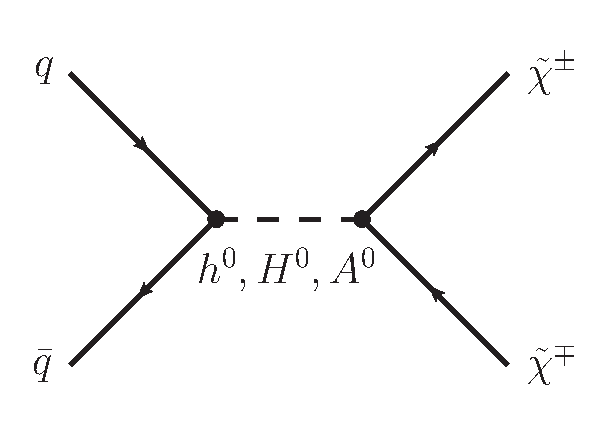
\includegraphics[width=0.33\textwidth]{figures/analysis/ChiChi_Scalar.pdf}
    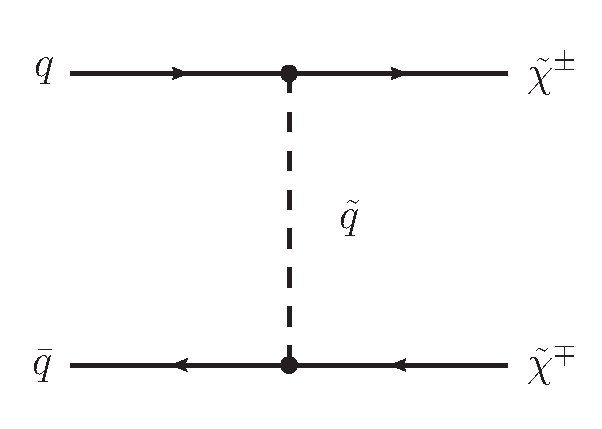
\includegraphics[width=0.33\textwidth]{figures/analysis/ChiChi_Squark.pdf}
  \end{tabular}
  \caption{Main tree level diagrams for chargino pair production.}
  \label{fig:FeynmanDiagramProductionCharginoPair}
\begin{tabular}{c}
    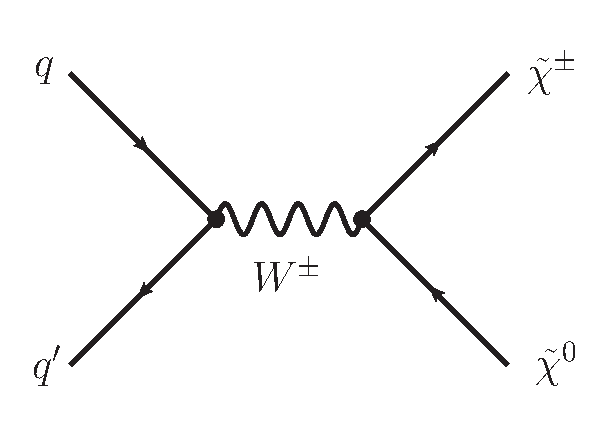
\includegraphics[width=0.33\textwidth]{figures/analysis/ChiChi0_WBoson.pdf}
    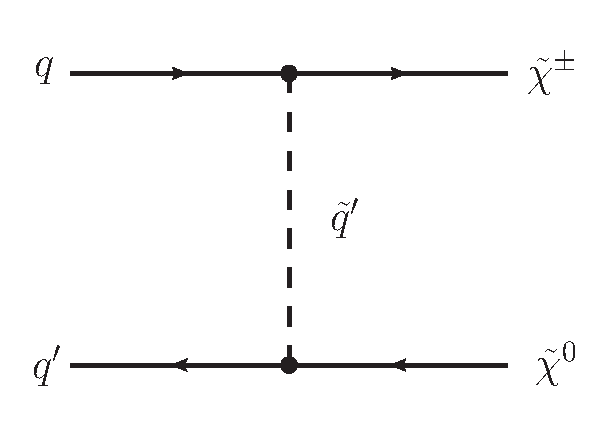
\includegraphics[width=0.33\textwidth]{figures/analysis/ChiChi0_Squark.pdf}
  \end{tabular}
  \caption{Main tree level diagrams for chargino neutralino production.}
  \label{fig:FeynmanDiagramProductionCharginoNeutralino}
\end{figure}
Another possibility of chargino production is the chargino neutralino production channel. 
On tree level, there exist two production mechanism: the s-channel W boson exchange and the t-channel squark exchange, see Fig.~\ref{fig:FeynmanDiagramProductionCharginoNeutralino} for the Feynman diagrams.\\

Even if the presented supersymmetric model where $\chi^{\pm}_1$ and $\chi^{0}_1$ are nearly mass-degenerate leads to more exotic signatures at the CMS experiment, there have been already several analyses conducted in CMS which are in principle (even not all were designed to be) sensitive to these models.
Among those are a search for long-lived charged particles \cite{bib:CMS:HSCP_8TeV}, which was mainly designed for particles which have such a long lifetime that they travel through the full detector without decaying and a search for disappearing tracks \cite{bib:CMS:DT_8TeV} which looked for rather intermediate lifetimes, where the charginos decays already inside the tracker. 
Within \cite{bib:CMS:DT_8TeV}, a study was done, based on an interpretation exercise \cite{bib:CMS:HSCPReinterpreation_PAS} within the phenomenological MSSM (see Sec.~\ref{theorySUSY} for a detailed introduction to the pMSSM), which tests the exclusion power of various analyses done at CMS.

\begin{figure}[!b]
  \centering 
  \begin{tabular}{c}
    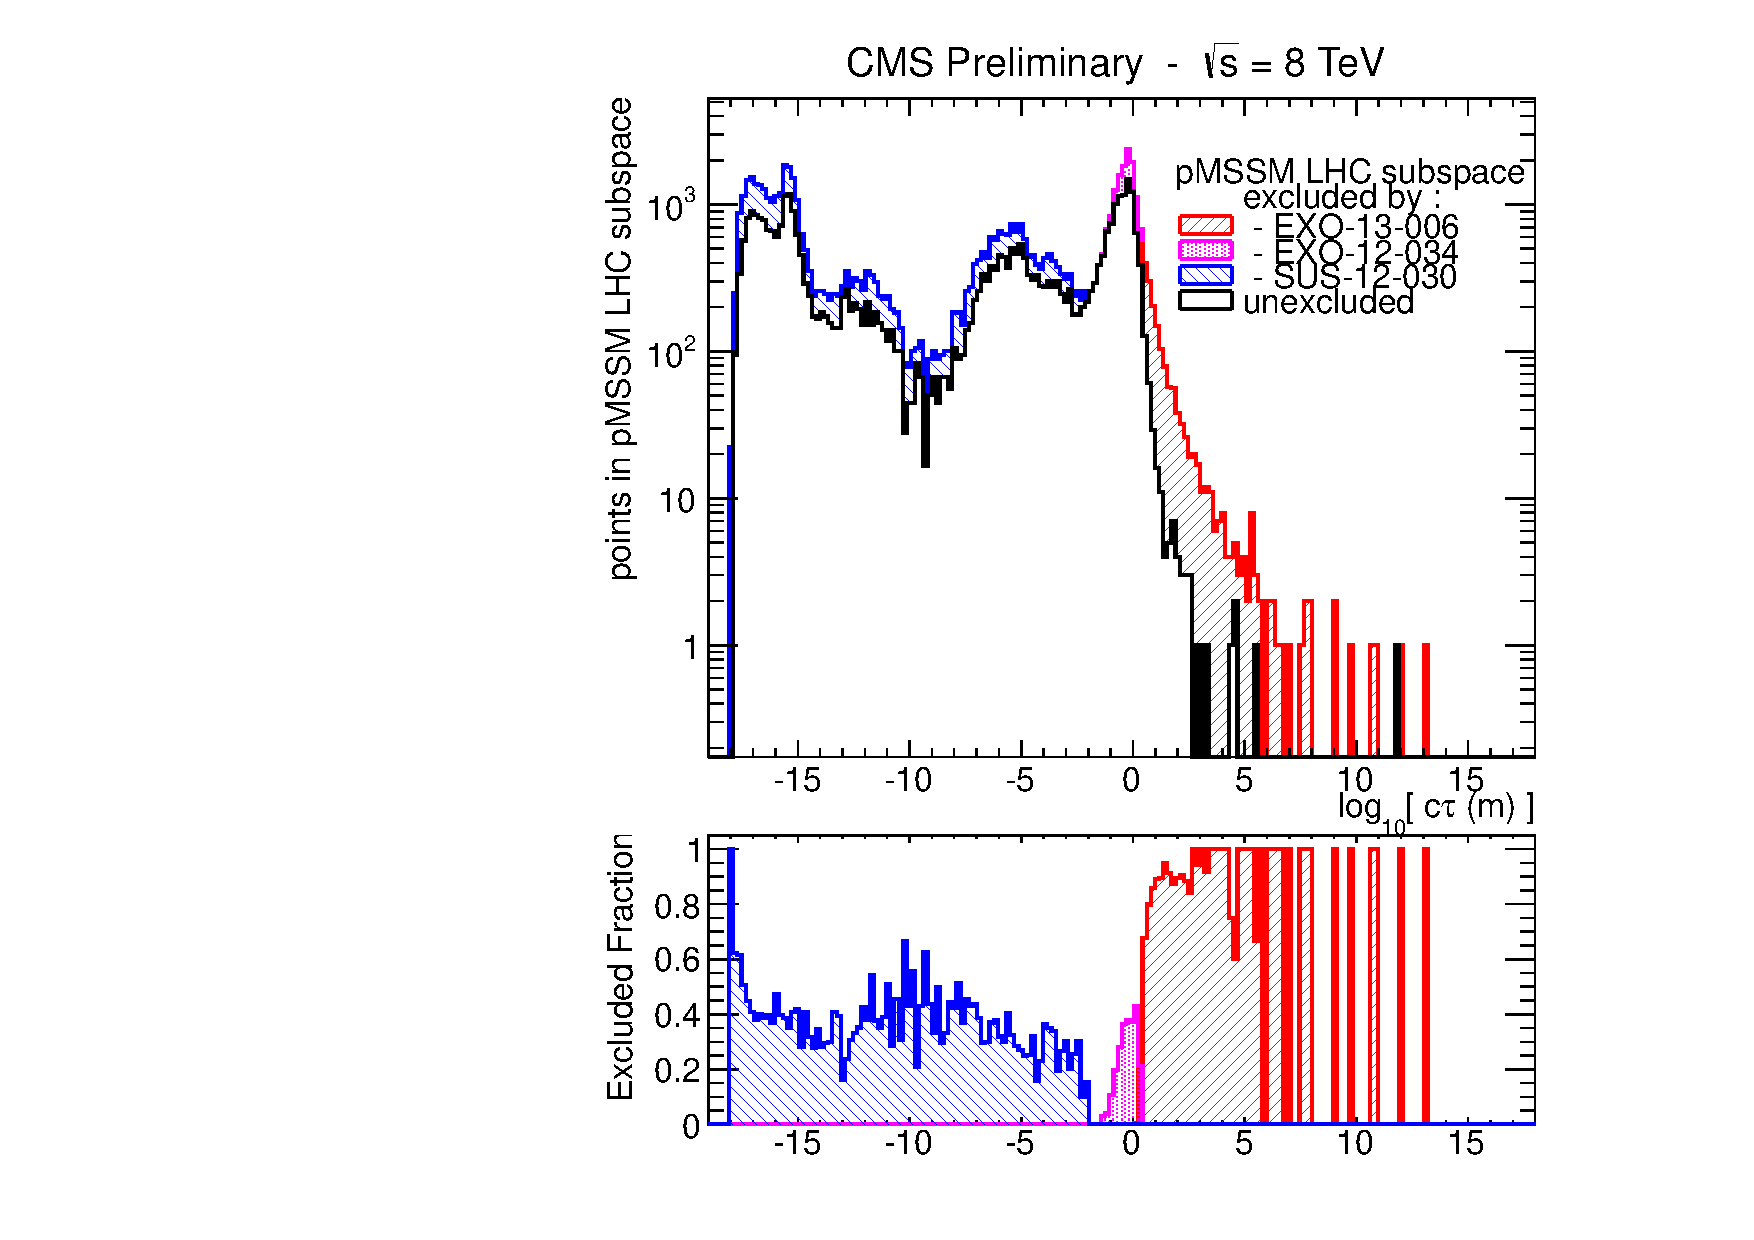
\includegraphics[width=0.75\textwidth]{figures/analysis/pMSSM_vs_ctau.pdf}
  \end{tabular}
  \caption{Exclusion power of various analyses dependent on chargino lifetime [c$\tau$]. Lower part of the plot shows the excluded fraction. Taken from: \href{https://twiki.cern.ch/twiki/bin/view/CMSPublic/PhysicsResultsEXO12034}{click here}.}
  \label{fig:pMSSMplot}
\end{figure}
In Fig.~\ref{fig:pMSSMplot}, the exclusion power of the search for long-live charged particles \cite{bib:CMS:HSCP_8TeV} in red, the search for diasappearing tracks \cite{bib:CMS:DT_8TeV} in purple and a collection of various SUSY analysis from \cite{bib:CMS:pMSSMinterpretation_7TeV_PAS} in blue over the chargino mass is shown. 
In black the distribution of the unexcluded pMSSM parameter points vs. the chargino mass can be seen.
The sampling of the parameter space points was done according to a pre-CMS likehood function, which takes into account electroweak precisicion measurements, etc.
In the lower part of Fig~\ref{fig:pMSSMplot}, the excluded fraction of pMSSM points is shown. 
It can be seen, that the more general SUSY searches are mostly sensitive to shorter chargino lifetimes ($c\tau \lesssim 10 \,\text{cm}$), whereas the search for long-lived particles shows very good sensitivity for lifetimes $>100\,$cm.
The search for disappearing tracks is sensitive on supersymmetric models with chargino lifetimes between $35\,\text{cm} \lesssim c\tau \lesssim 100\,\text{cm}$.

This analysis is targeting the gap between the disappearing track search (purple area) and the searches which are sensitive to instanteanously decaying charginos (blue area). The idea is to make use of the variable dE/dx which can be very discriminating for particles with high mass.
The challenges of such a search and the general strategy of this analysis will be presented int the next section.


%There are many analyses done at CMS which are in principle sensitive to such a supersymmetric chargino. 
%This analyis wants to focus on long lifetimes such that the chargino does not directly decay, but reaches at least to first layers of the detector, being the silicon pixel and strip trackers. 
%On the other hand, it has been designed in a way, that the chargino is not that-lonmg lived, that it travels through the whole detector, but decays at least before the muon chambers, thus is not reconstructed as a muon.
%There have been analysis at CMS and Atlas looking for such middel-live charginos. 
%The new aspect of the analysis is the inclusion of the variable dE/dx.
%The pixel and the silicon tracker at CMS have been calibrated already offline, when building these moduls. Unfortunately it is not so good.
%The silicon strip tracker has been calibrated in the context of a search for heavy, stable charged particle (cite something).
%In this analysis, also very short tracks become very important, showing not more than three of four hits. Therfore also the pixel detector needs to bec calibrated in order to increase senssitivy for those short tracks


%%%%%%%%%%%%%%%%%%%%%%%%%%%%%%%%%%%%%%%%%%%%%%%%%%%%%%%%%%%%%%%%%%%%%%%%%%%%%%%%%%%%%%%%%%%%%%%%%%%%%%%%%%%%%%%%%%%%%%%%%%%%%%%%%%%%%%%%%%%%%%%%%%%%%%%%%%%%%%%%%%%%%%%%%%%%%%%%%%%%
\section{General search strategy}
\label{sec:GeneralSearchStrategy}

When searching for supersymmetric models with long-lived \chipm, the strategy is of course highly dependent on the actual lifetime of the chargino. 
For long lifetimes, the chargino can reach the muon chambers and can be reconstructed as a muon (even with a longer time-of-flight). 
For lower lifetimes, the chargino can already decay inside the detector (e.g. the tracker), thus not leading a reconstructed muon in the event, but only to an isolated track in the tracker. 
The detector signatures of these two scenarios are visualised in Fig~\ref{fig:CharginoPaiEventDisplay}, where in a cross-sectional view of the CMS detector simulated chargino-chargino events are shown.
\begin{figure}[!b]
  \centering 
  \begin{tabular}{c}
    \frame{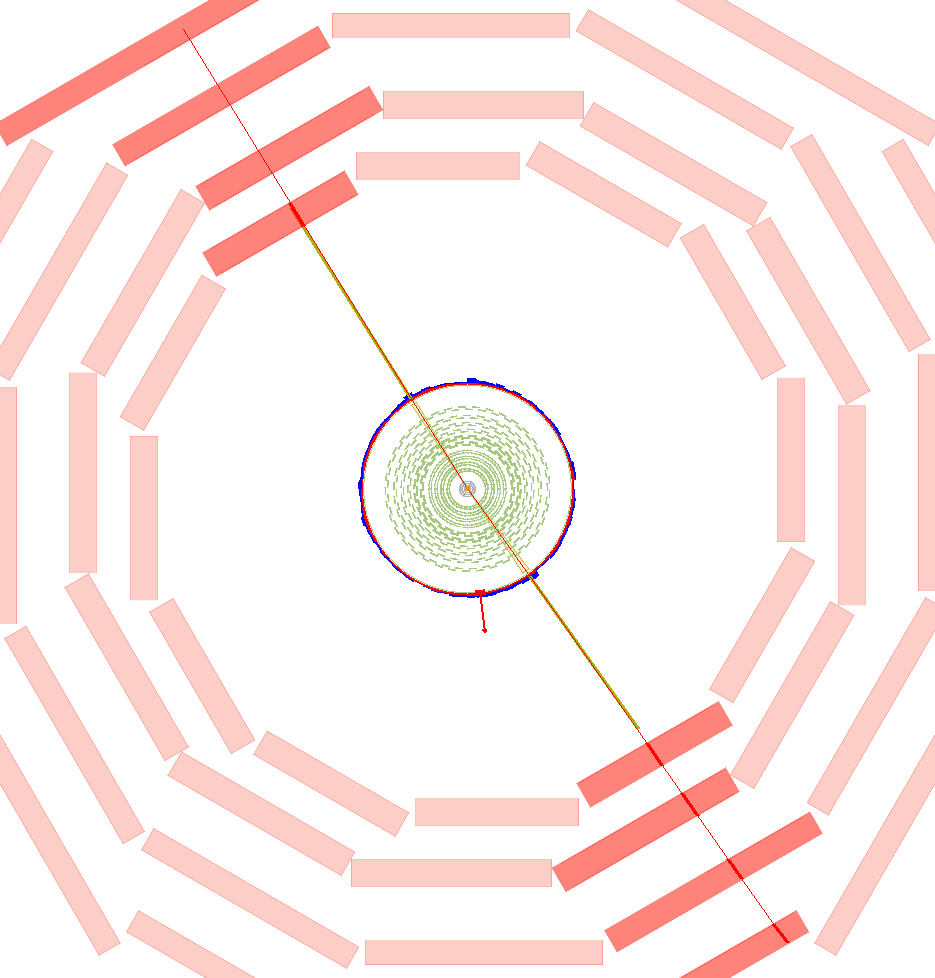
\includegraphics[width=0.31\textwidth]{figures/analysis/EventDisplay_scenario1.png}}
    \frame{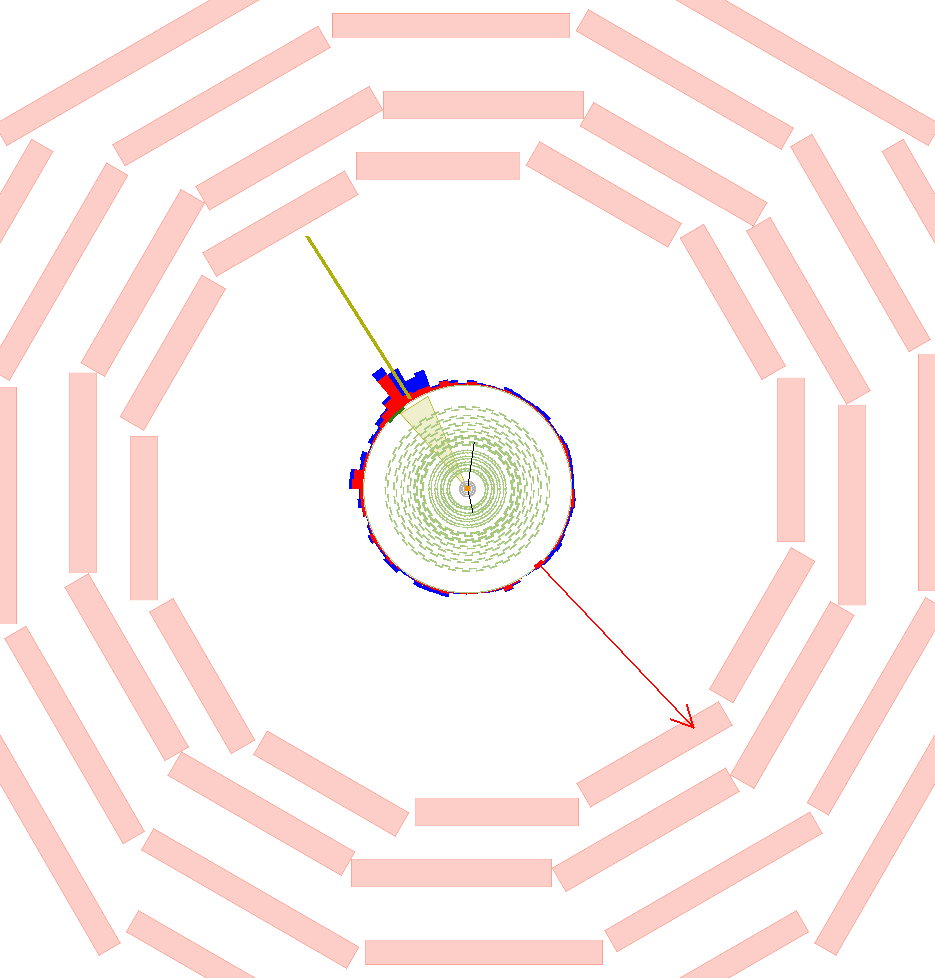
\includegraphics[width=0.31\textwidth]{figures/analysis/EventDisplay_scenario2.png}}
    \frame{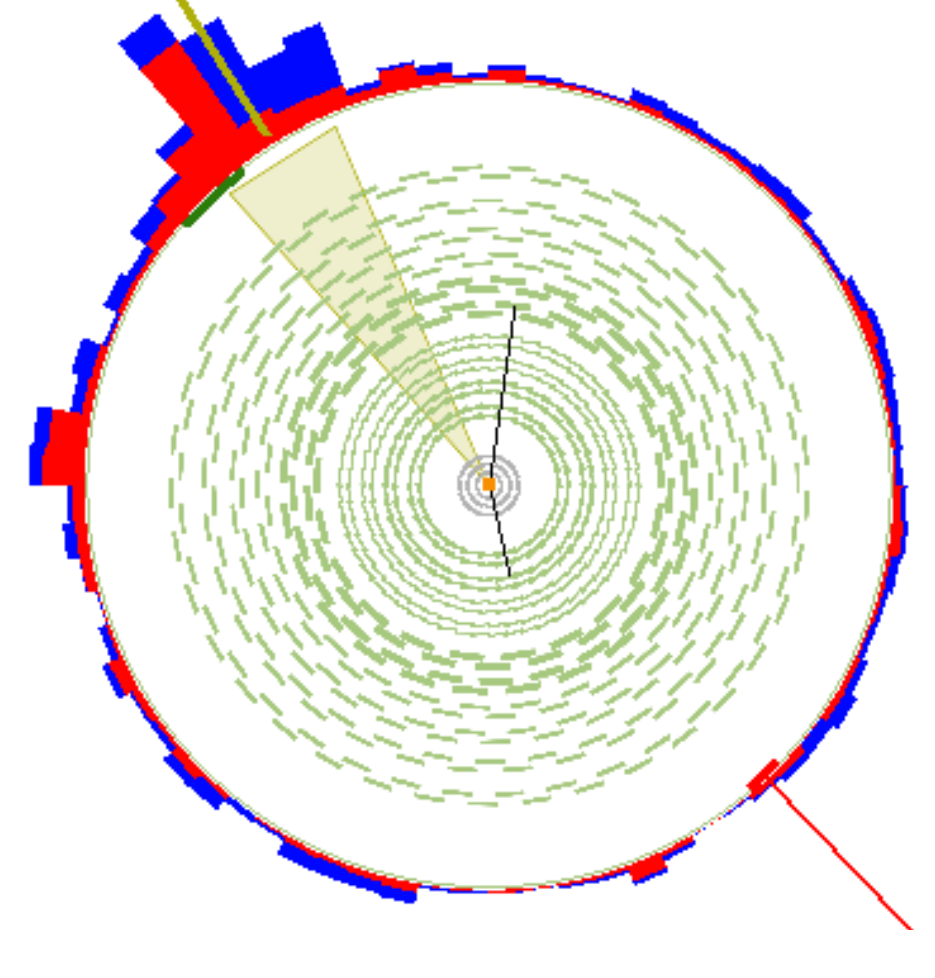
\includegraphics[width=0.31\textwidth]{figures/analysis/EventDisplay_scenario2_Zoomed.png}}
  \end{tabular}
  \caption{Visualisation of possible signatures of a chargino pair produced with a lifetime of $c\tau = 10\,\text{m}$ (left) and a lifetime of $c\tau = 0.5\,\text{m}$ (middle and right). 
           In the left picture, both charginos are reconstructed as muons, which can be seen in the energy deposition in the muon chambers (red boxes). 
           In the middle picture both charginos are only visible as tracks in the tracker (black lines), where both trajectories end inside the silicon tracker, showing the decay point point of the corresponding chargino. 
           The right picture is a zoom of the picture in the middle. Here only the cross-section of the tracker (green wavy lines) is displayed. The red arrow shows the missing transverse energy in the event.} 
  \label{fig:CharginoPaiEventDisplay}
\end{figure}
As mentioned before, this analysis targets a search for supersymmetry with charginos of lifetimes between $10\,\text{cm} \lesssim c\tau \lesssim  40\,\text{cm}$.
That means that the charginos decay rather early in the detector, even at the beginning of the tracker. 
The distinct challenges of such an analysis, shall be listed in the following passage.

First of all, in case R-parity (see Sec.~\ref{theorySUSY}) is conserved, one of the decay products of the chargino, which is the lightest neutralino \chiO is stable, thus travelling through the whole detector only weakly intereacting.
Therefore it is not detectable. 
The other chargino decay product, e.g. a pion, can be hardly reconstructed, mainly because it does not origin from the primary vertex (if the chargino reaches the detector before its decay), 
but secondarily because it is very low in momentum because of the mass-degeneracy between \chipm and \chiO.
The momentum of the decay product is of course highly dependent on the actual mass gap between the neutralino and the chargino.
A typical \pt distribution of a pion originating from a chargino decay can be found in Fig.~\ref{fig:KinkedTrack} for a mass gap between \chipm and \chiO of 150\,\mev.
\begin{figure}[!t]
  \centering 
  \begin{tabular}{c}
    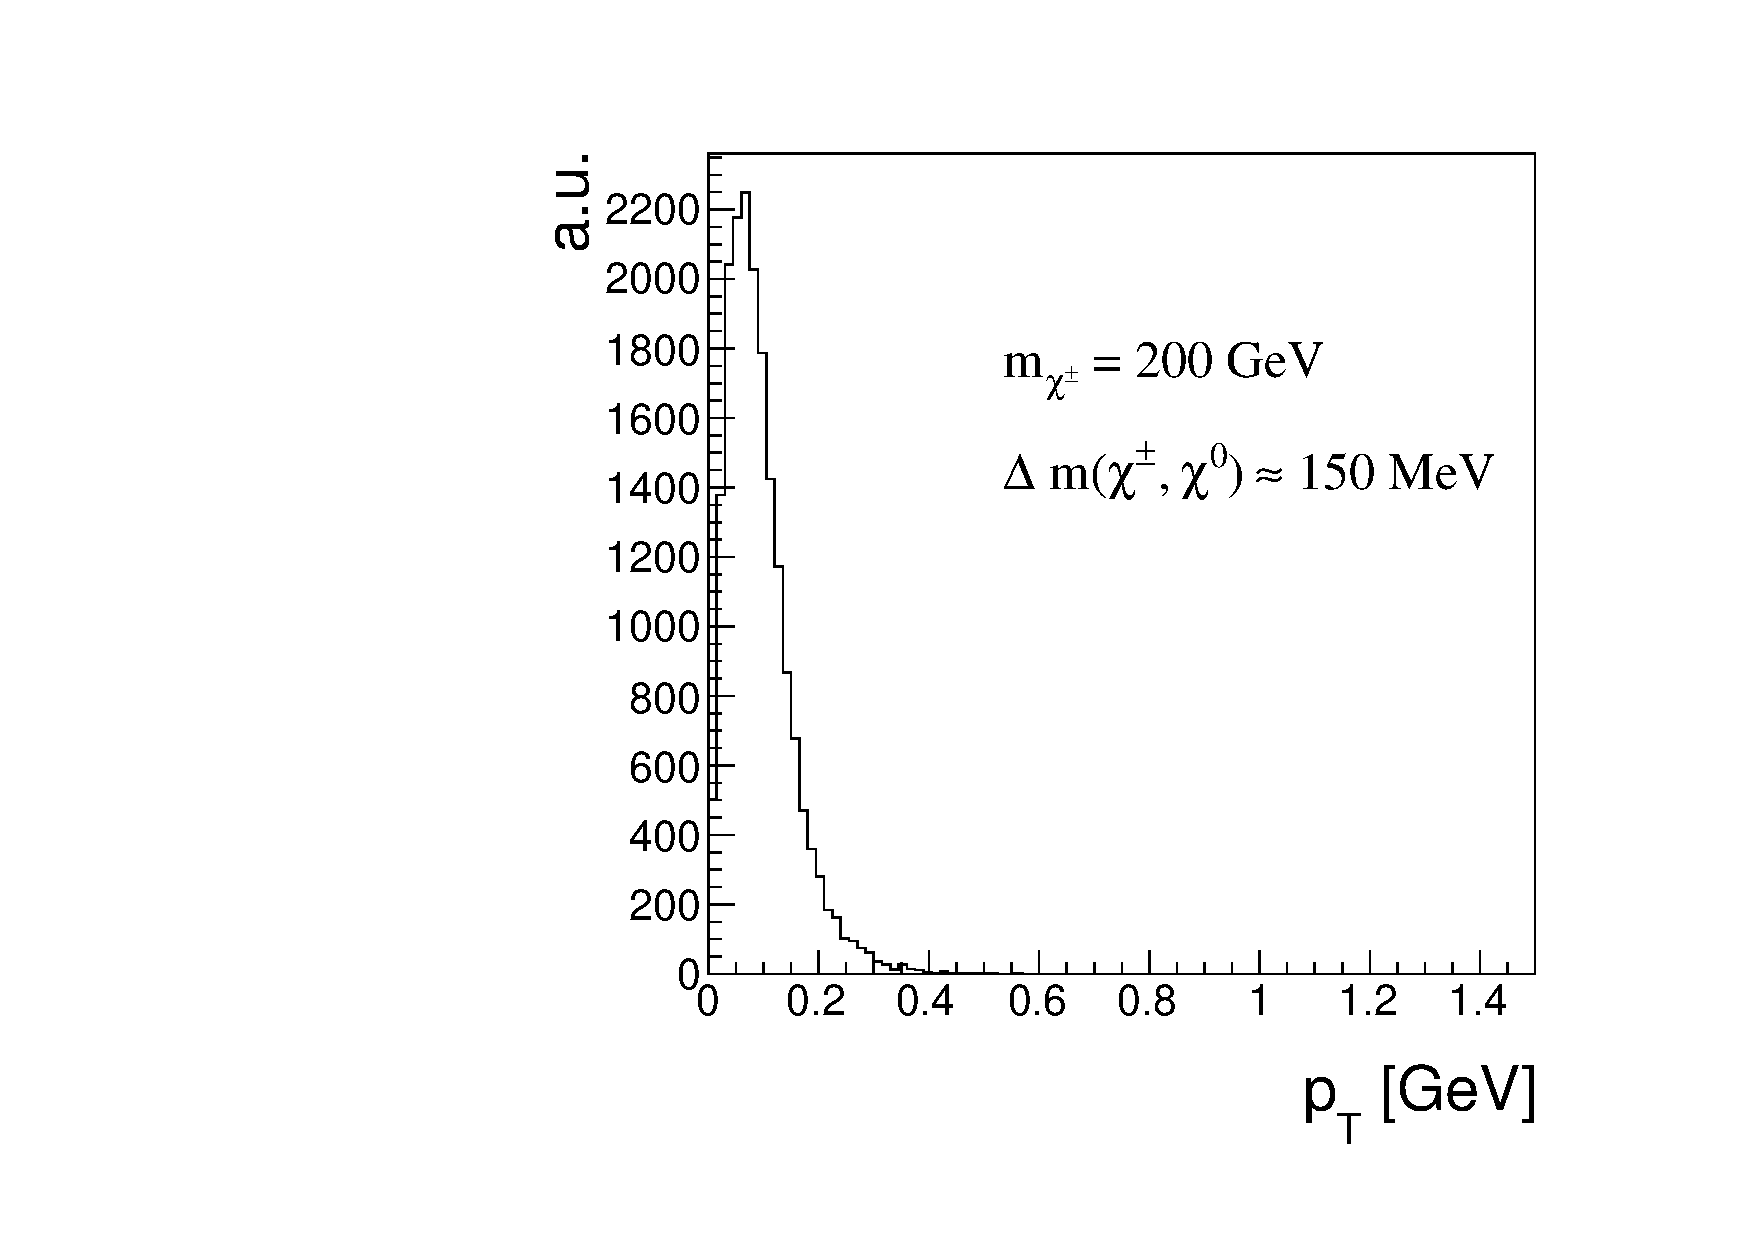
\includegraphics[width=0.6\textwidth]{figures/analysis/ptOfPions.pdf}
  \end{tabular}
  \caption{Transverse momentum distribution of pions coming from chargino decay into a neutralino with a mass gap of 150\mev.}
  \label{fig:ptOfPions}
\end{figure} 
The \pt distribution peaks at \mbox{$\sim$ 100\,\mev} and ends at \mbox{\pt $\sim 400\,$\mev}.
When the transverse momentum of a particle is very low, the particle trajectory is much more bended compared to a particle with higher \pt (see Fig.~\ref{fig:KinkedTrack} for illustration), 
thus making the detection of such a particle very challinging.
\begin{figure}[!bt]
  \centering 
  \begin{tabular}{c}
    \frame{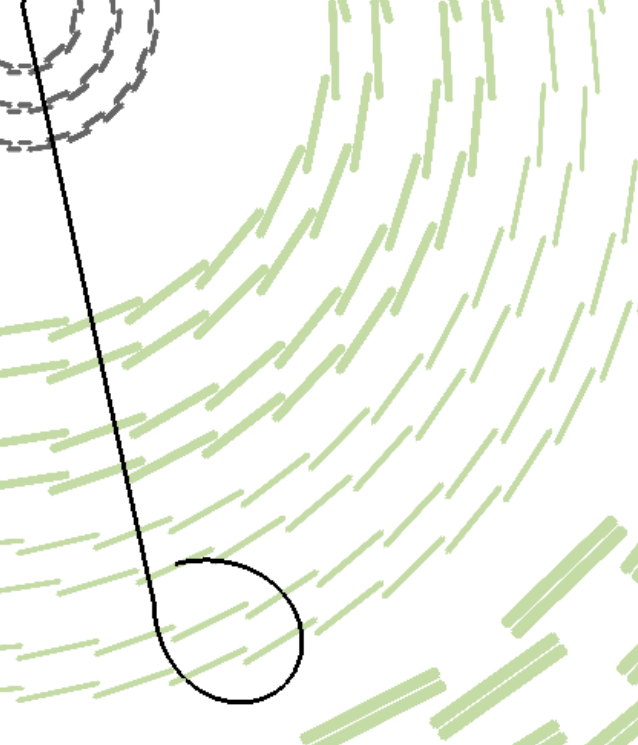
\includegraphics[width=0.3\textwidth]{figures/analysis/KinkedTrackZoom.png}}
  \end{tabular}
  \caption{Cross-sectional view of the tracker (different tracker layers are illustrated with wavy green lines) and a simulated chargino track (black line) decays to a pion (bended black line).}
  \label{fig:KinkedTrack}
\end{figure} 
Because of the stronger bending, the track reconstruction efficiency decreases for particles with a transverse momentum below 1\,\gev rapidely, ending at around 40\% for isolated pions with a \pt of 100\mev (see \cite{bib:CMS:tracking_8TeV}).

Taking the hard or even impossible detection of the decay products of the chargino, this lead to the fact, that besides the (short) track of the chargino, nothing can be seen in the detector.
Unfortunately, there is no dedicated track trigger at CMS, which makes a specific detection of those events with the help of the chargino track impossible.
To be able to search for these models, one therefore need to take advantage of higher order contributions to the feynman diagrams shown in the previous sections (Figs.~\ref{fig:FeynmanDiagramProductionCharginoPair},\ref{fig:FeynmanDiagramProductionCharginoNeutralino}), resulting in initial state radiation.
When the initial quarks radiate a high \pt gluon, the resulting jet can be detected and offering a possibility to search for isolated tracks in the tracker.






\begin{itemize}
%\item No detection of low momentum fermions possible (fermion pt plot?), no detection of the decay products
%\item Concentration on intermediate lifetime $\rightarrow$ only a (short) chargino track can be seen.
%\item Show event displays and sketch for pion decyay!
\item Detection via ISR 
\item Event selection by ISR jet and MET
\item Detection of track (possibly short and disappearing and highly ionizing, not reconstructed as muon)
\item Short and highly ionizing track $\rightarrow$ inclusion of pixel tracker information 
\end{itemize}



\subsection{Comparison to existing searches}
\begin{itemize}
\item HSCP
\item Disappearing track
\item No cut on Nhits
\item Muon veto + inclusion of dE/dx
\end{itemize}

%%%%%%%%%%%%%%%%%%%%%%%%%%%%%%%%%%%%%%%%%%%%%%%%%%%%%%%%%%%%%%%%%%%%%%%%%%%%%%%%%%%%%%%%%%%%%%%%%%%%%%%%%%%%%%%%%%%%%%%%%%%%%%%%%%%%%%%%%%%%%%%%%%%%%%%%%%%%%%%%%%%%%%%%%%%%%%%%%%%%
\section{(Improved) dE/dx measurement of short tracks}
\label{sec:DeDxMeasurement}
\subsection{Measuring dE/dx}
\begin{itemize}
\item The variable dE/dx: General introdution, Bethe-Bloch, 
\item Asymmetric Smirnov Discriminator
\end{itemize}
\subsection{Gain calibration of the silicon pixel tracker}
\subsection{Asymmetric Smirnov discriminator}
\subsection{Efficiency improvements}

%%%%%%%%%%%%%%%%%%%%%%%%%%%%%%%%%%%%%%%%%%%%%%%%%%%%%%%%%%%%%%%%%%%%%%%%%%%%%%%%%%%%%%%%%%%%%%%%%%%%%%%%%%%%%%%%%%%%%%%%%%%%%%%%%%%%%%%%%%%%%%%%%%%%%%%%%%%%%%%%%%%%%%%%%%%%%%%%%%%%
\section{Simulated samples}
\label{sec:SimulatedSamples}
\subsection{SM samples}
\subsection{Signal samples}

%%%%%%%%%%%%%%%%%%%%%%%%%%%%%%%%%%%%%%%%%%%%%%%%%%%%%%%%%%%%%%%%%%%%%%%%%%%%%%%%%%%%%%%%%%%%%%%%%%%%%%%%%%%%%%%%%%%%%%%%%%%%%%%%%%%%%%%%%%%%%%%%%%%%%%%%%%%%%%%%%%%%%%%%%%%%%%%%%%%%
\section{Event selection}
\label{sec:EventSelection}
\subsection{Datasets and triggers}
\begin{itemize}
\item Datasets and triggers used in the analysis
\item signal samples generated with Madgraph and pythia
\item They are decayed in Geant to only pions. Around ten different lifetimes were simulated
\item For other lifetimes: lifetime reweighting is done PLOT
\item For five diffenrent masses (100-500 GeV) 
\end{itemize}
\subsection{Preselection}
\begin{itemize}
\item Motivate different selection cuts
\item Reference DT search for most of them
\end{itemize}
\subsection{Main discriminating variables}
\begin{itemize}
\item dE/dx
\item pt
\item Show some MC signal bkg comparioson plots (only Wjets?)
\end{itemize}

%%%%%%%%%%%%%%%%%%%%%%%%%%%%%%%%%%%%%%%%%%%%%%%%%%%%%%%%%%%%%%%%%%%%%%%%%%%%%%%%%%%%%%%%%%%%%%%%%%%%%%%%%%%%%%%%%%%%%%%%%%%%%%%%%%%%%%%%%%%%%%%%%%%%%%%%%%%%%%%%%%%%%%%%%%%%%%%%%%%%
\section{Sources of backgrounds}
\label{sec:SourcesOfBackgrounds}
\begin{itemize}
\item Background consist of particles which make high energy deposits and are high pt
\item In general: Low background search
\end{itemize}
\subsection{Fake tracks}
\begin{itemize}
\item Definition of fake tracks
\item How can they fake the signal
\end{itemize}
\subsection{Muons}
\begin{itemize}
\item How can muons fake the signal
\end{itemize}
\subsection{Pions}
\begin{itemize}
\item How can pions fake the signal
\end{itemize}
\subsection{Electrons}
\begin{itemize}
\item How can electrons fake the signal
\end{itemize}

%%%%%%%%%%%%%%%%%%%%%%%%%%%%%%%%%%%%%%%%%%%%%%%%%%%%%%%%%%%%%%%%%%%%%%%%%%%%%%%%%%%%%%%%%%%%%%%%%%%%%%%%%%%%%%%%%%%%%%%%%%%%%%%%%%%%%%%%%%%%%%%%%%%%%%%%%%%%%%%%%%%%%%%%%%%%%%%%%%%%
\section{Background estimation methods}
\label{sec:BackgroundEstimation}
\subsection{Fake background}
\subsection{Leptonic background}
\subsection{Systematic uncertainties}

%%%%%%%%%%%%%%%%%%%%%%%%%%%%%%%%%%%%%%%%%%%%%%%%%%%%%%%%%%%%%%%%%%%%%%%%%%%%%%%%%%%%%%%%%%%%%%%%%%%%%%%%%%%%%%%%%%%%%%%%%%%%%%%%%%%%%%%%%%%%%%%%%%%%%%%%%%%%%%%%%%%%%%%%%%%%%%%%%%%%
\section{Optimization of search sensitivity}
\label{sec:Optimization}
\begin{itemize}
\item Show plots
\item show table
\item Include NlostOuter here, too
\end{itemize}

%%%%%%%%%%%%%%%%%%%%%%%%%%%%%%%%%%%%%%%%%%%%%%%%%%%%%%%%%%%%%%%%%%%%%%%%%%%%%%%%%%%%%%%%%%%%%%%%%%%%%%%%%%%%%%%%%%%%%%%%%%%%%%%%%%%%%%%%%%%%%%%%%%%%%%%%%%%%%%%%%%%%%%%%%%%%%%%%%%%%
\section{Statistical Methods/ Limit setting}
\label{sec:LimitSetting}

%%%%%%%%%%%%%%%%%%%%%%%%%%%%%%%%%%%%%%%%%%%%%%%%%%%%%%%%%%%%%%%%%%%%%%%%%%%%%%%%%%%%%%%%%%%%%%%%%%%%%%%%%%%%%%%%%%%%%%%%%%%%%%%%%%%%%%%%%%%%%%%%%%%%%%%%%%%%%%%%%%%%%%%%%%%%%%%%%%%%
\section{Results}
\label{sec:Results}
\begin{itemize}
\item Data cutflowtable
\item Tables with results
\item One plot (4 bins: Prediction and data)
\end{itemize}

%%%%%%%%%%%%%%%%%%%%%%%%%%%%%%%%%%%%%%%%%%%%%%%%%%%%%%%%%%%%%%%%%%%%%%%%%%%%%%%%%%%%%%%%%%%%%%%%%%%%%%%%%%%%%%%%%%%%%%%%%%%%%%%%%%%%%%%%%%%%%%%%%%%%%%%%%%%%%%%%%%%%%%%%%%%%%%%%%%%%
\section{Interpretation}
\label{sec:Interpretation}
\subsection{Systematic uncertainties of simulated signal samples}
\subsection{Exclusion limits}
\begin{itemize}
\item 1-d limits
\item 2-d limits
\end{itemize}

